% !TeX root = Introduction.tex
%% ^^^^^^^^^^^^^^^^^^^^^^^^^^ Change to match title of file
%% ----------------------------------------------------------------
%% Introduction.tex
%% ---------------------------------------------------------------- 

\documentclass[../main/Progress.tex]{subfiles}

%TODO uncomment the bib resource if you want autocomplete for references. Remember to comment it out before compiling your main document.
%\addbibresource{../Bibliography/biblio.bib} 

\begin{document}
	\chapter[Sample Chapter]{Sample Chapter}
	\section{Sample section}
	\subsection{Sample subsection}
	Some text. 
	Change of line.\\
	Sample citation~\cite{Fiat:1987}. 
	A sample image below:
	\begin{figure}[h]
		\centering
		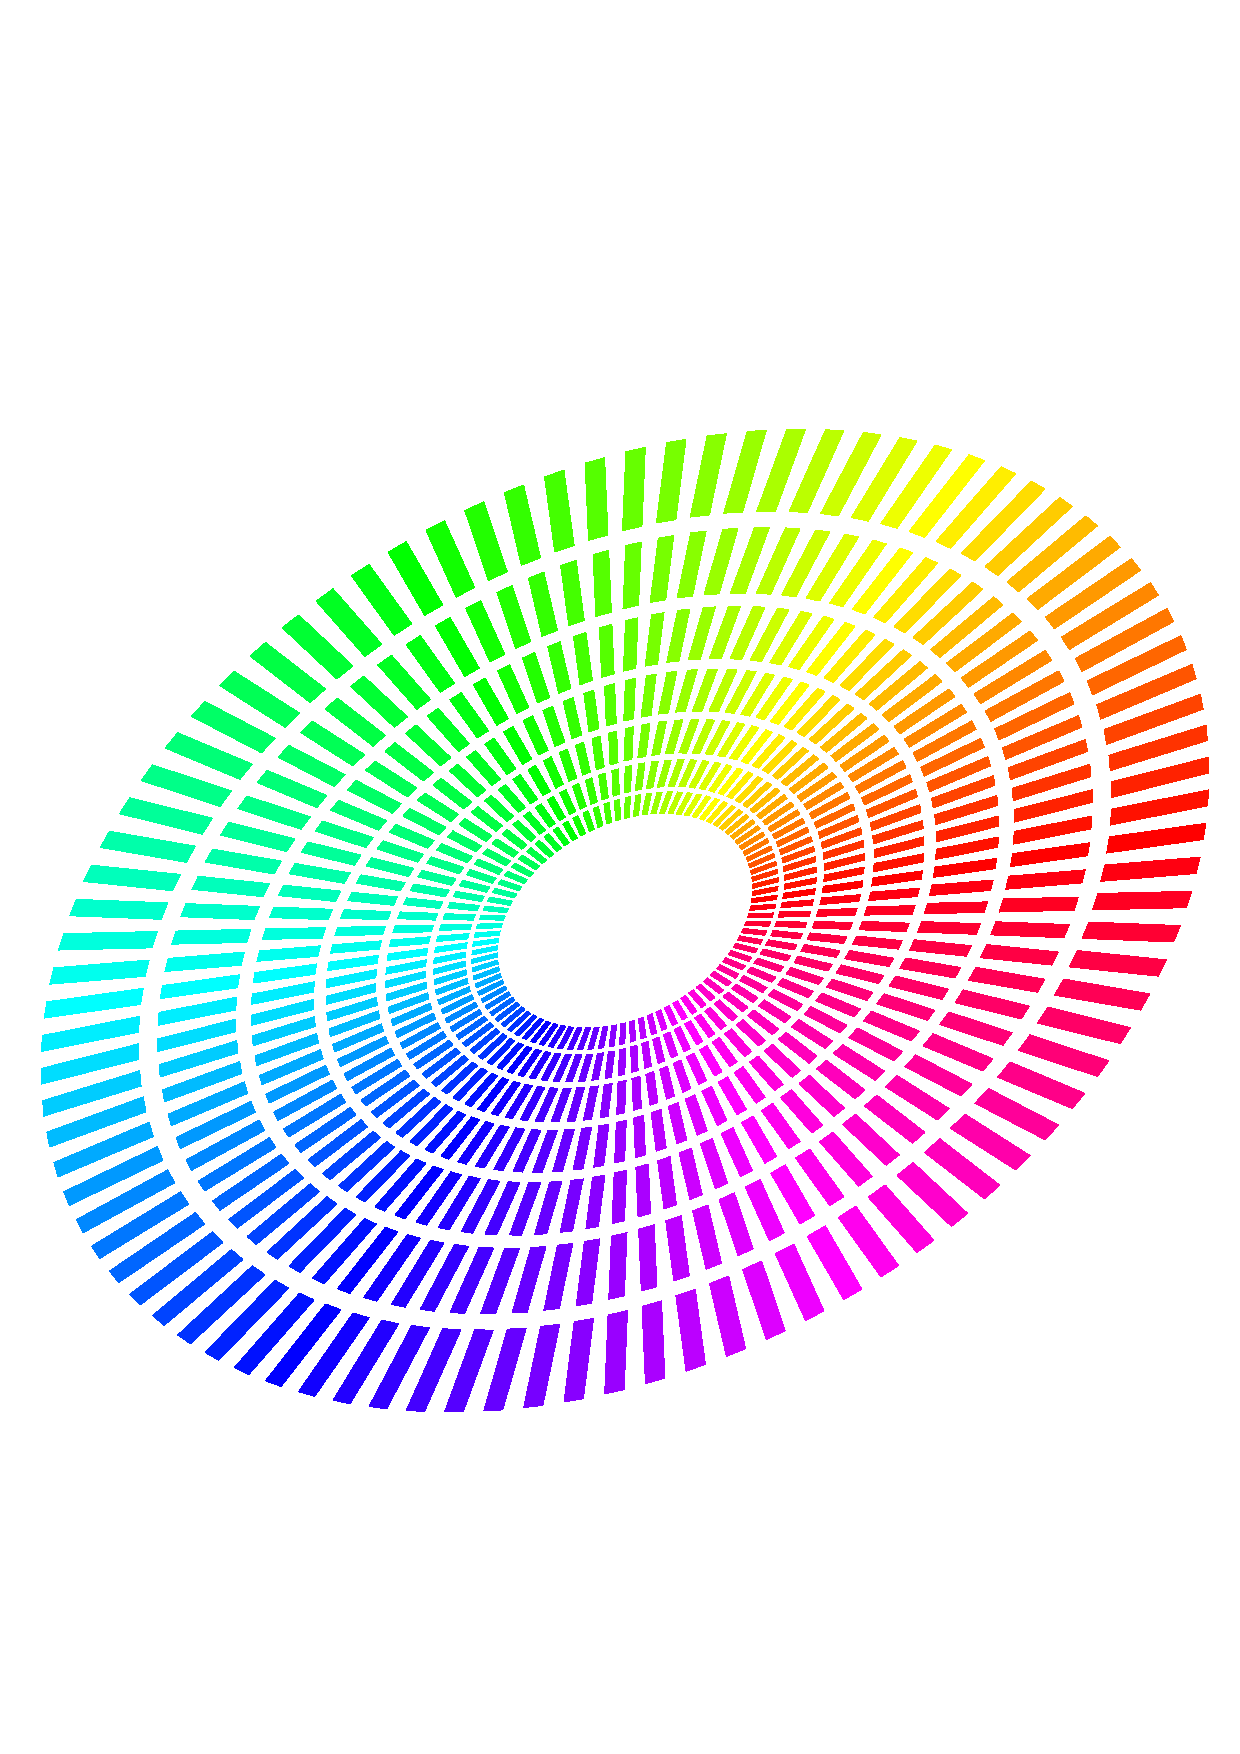
\includegraphics[width=0.5\linewidth]{figure}
		\caption[How the caption will appear in the list of figures]{How the caption will be in text. Here citations can be included \cite{Fiat:1987}.}
		\label{fig:figure}
	\end{figure}


This is how the default reference command \verb|\ref{fig:figure}| outputs cross-references: \ref{fig:figure}.\\
Using the \verb|cleveref| package, cross-referencing can be smarter. 
Here's the same reference, but using the command \verb|\cref{fig:figure}|: \cref{fig:figure}.
Or, using \verb|\Cref{fig:figure}|: \Cref{fig:figure}.


	
\end{document}